% Two-dimensional functions show the full landscape; higher-dimensional functions show a slice.
\begin{figure}[p]
  \begin{adjustwidth}{-\extralength}{0cm}
  \centering
  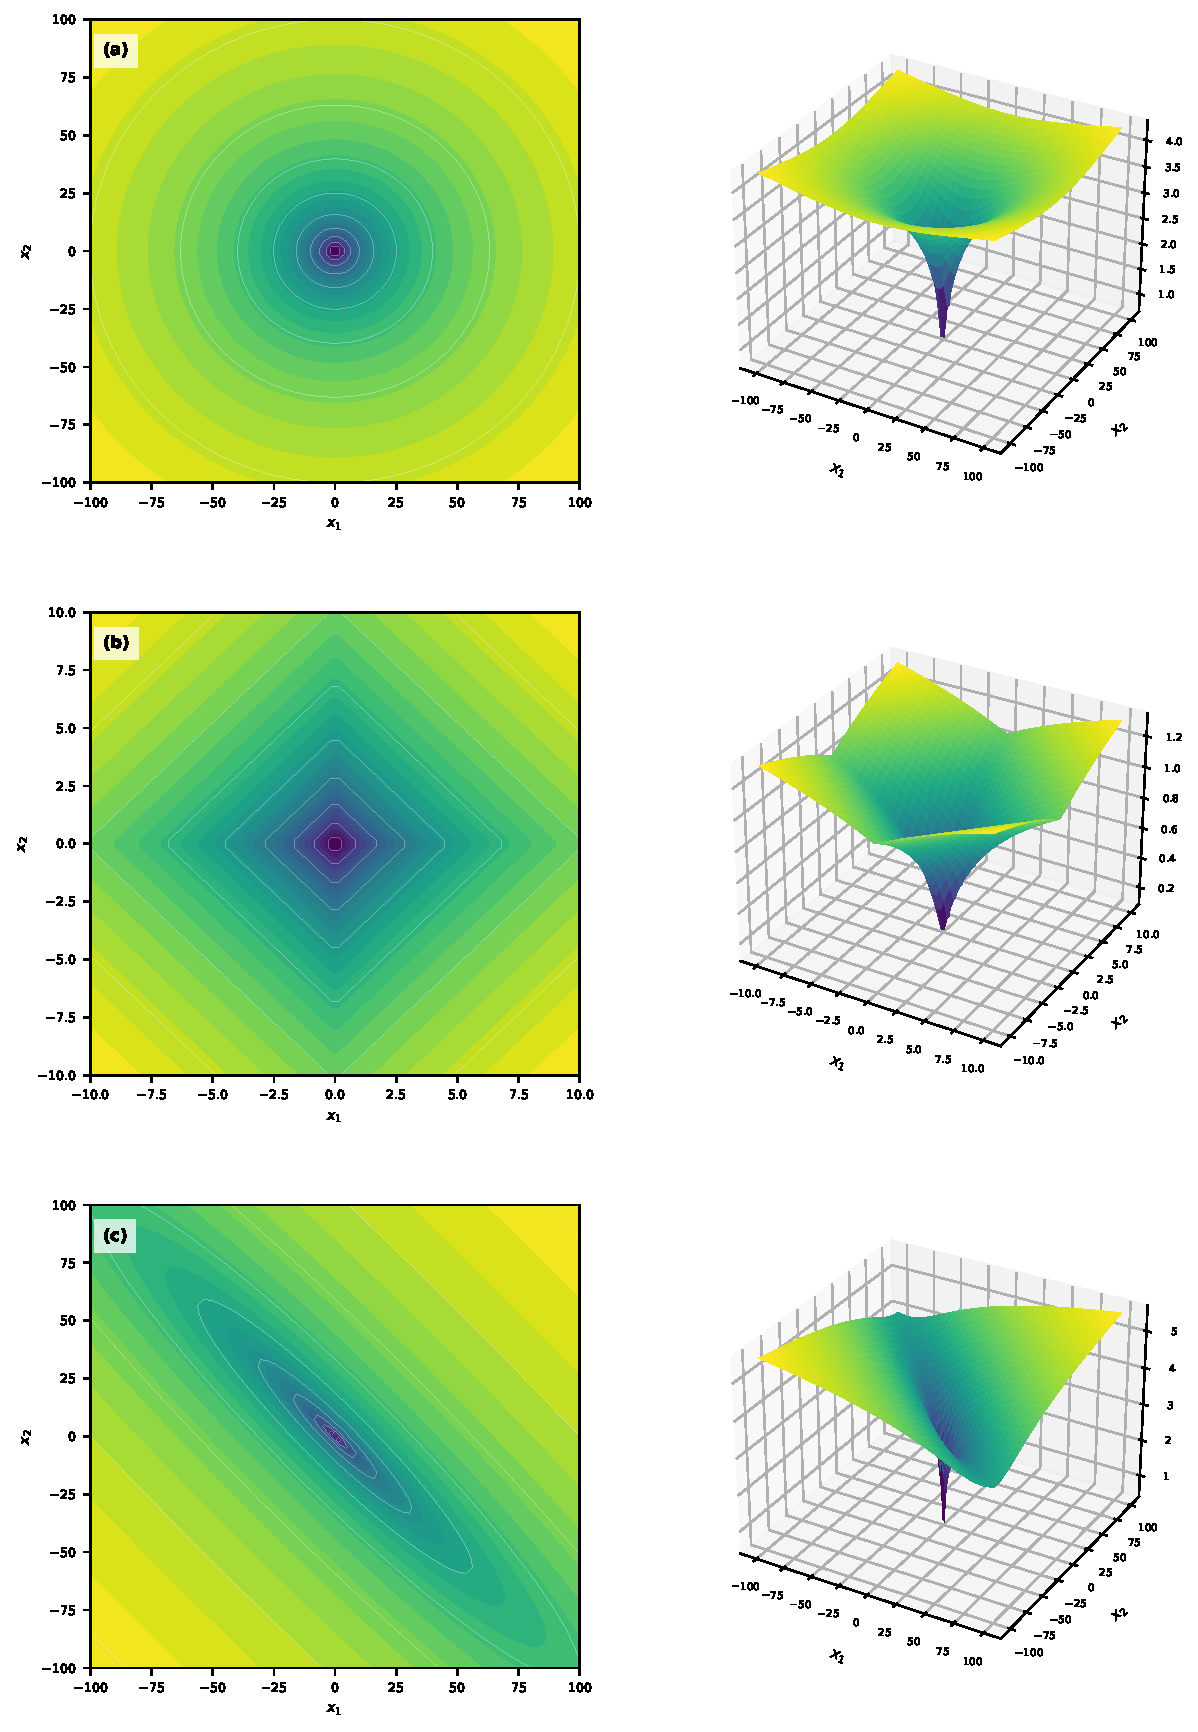
\includegraphics[width=\fulllength,height=0.84\textheight,keepaspectratio]{figures/landscapes_body/landscape_body_group_01.pdf}
  \end{adjustwidth}
  \caption{Benchmark objective landscapes and two-dimensional slices: (a) F1 (Sphere, $d=10$); (b) F2 (Schwefel 2.22, $d=10$); (c) F3 (Schwefel 1.2, $d=10$). Contours are shown at left and 3-D surfaces at right; colour shows log-compressed objective excess on function-specific scales. For $d>2$, other coordinates are fixed at the midpoint of the solver bounds. Bounds and reference optima are listed in Tables~\ref{tab:benchmark_scalable}--\ref{tab:benchmark_fixed}.}
  \label{fig:landscape_body_01}
\end{figure}
\clearpage

\begin{figure}[p]
  \begin{adjustwidth}{-\extralength}{0cm}
  \centering
  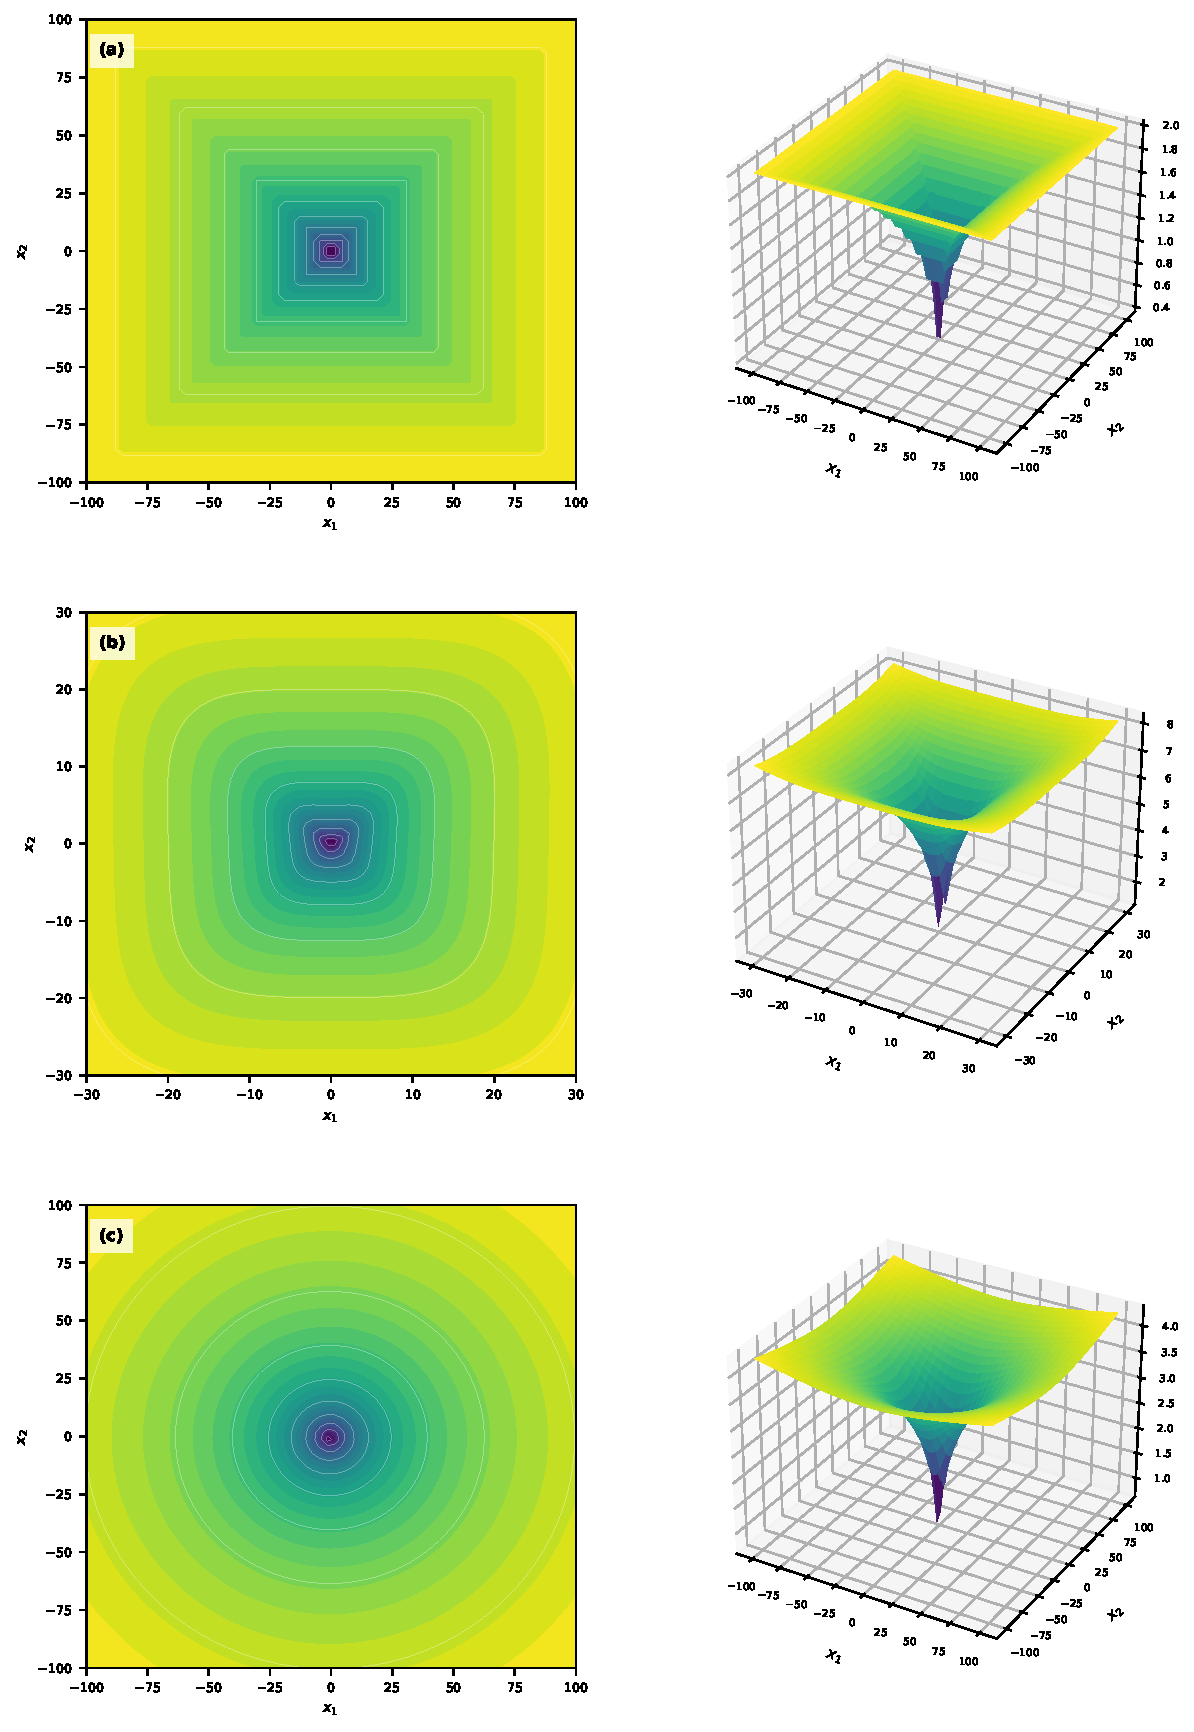
\includegraphics[width=\fulllength,height=0.84\textheight,keepaspectratio]{figures/landscapes_body/landscape_body_group_02.pdf}
  \end{adjustwidth}
  \caption{Benchmark objective landscapes and two-dimensional slices: (a) F4 (Schwefel 2.21, $d=10$); (b) F5 (Rosenbrock, $d=10$); (c) F6 (Shifted step, $d=10$). Contours are shown at left and 3-D surfaces at right; colour shows log-compressed objective excess on function-specific scales. For $d>2$, other coordinates are fixed at the midpoint of the solver bounds. Bounds and reference optima are listed in Tables~\ref{tab:benchmark_scalable}--\ref{tab:benchmark_fixed}.}
  \label{fig:landscape_body_02}
\end{figure}
\clearpage

\begin{figure}[p]
  \begin{adjustwidth}{-\extralength}{0cm}
  \centering
  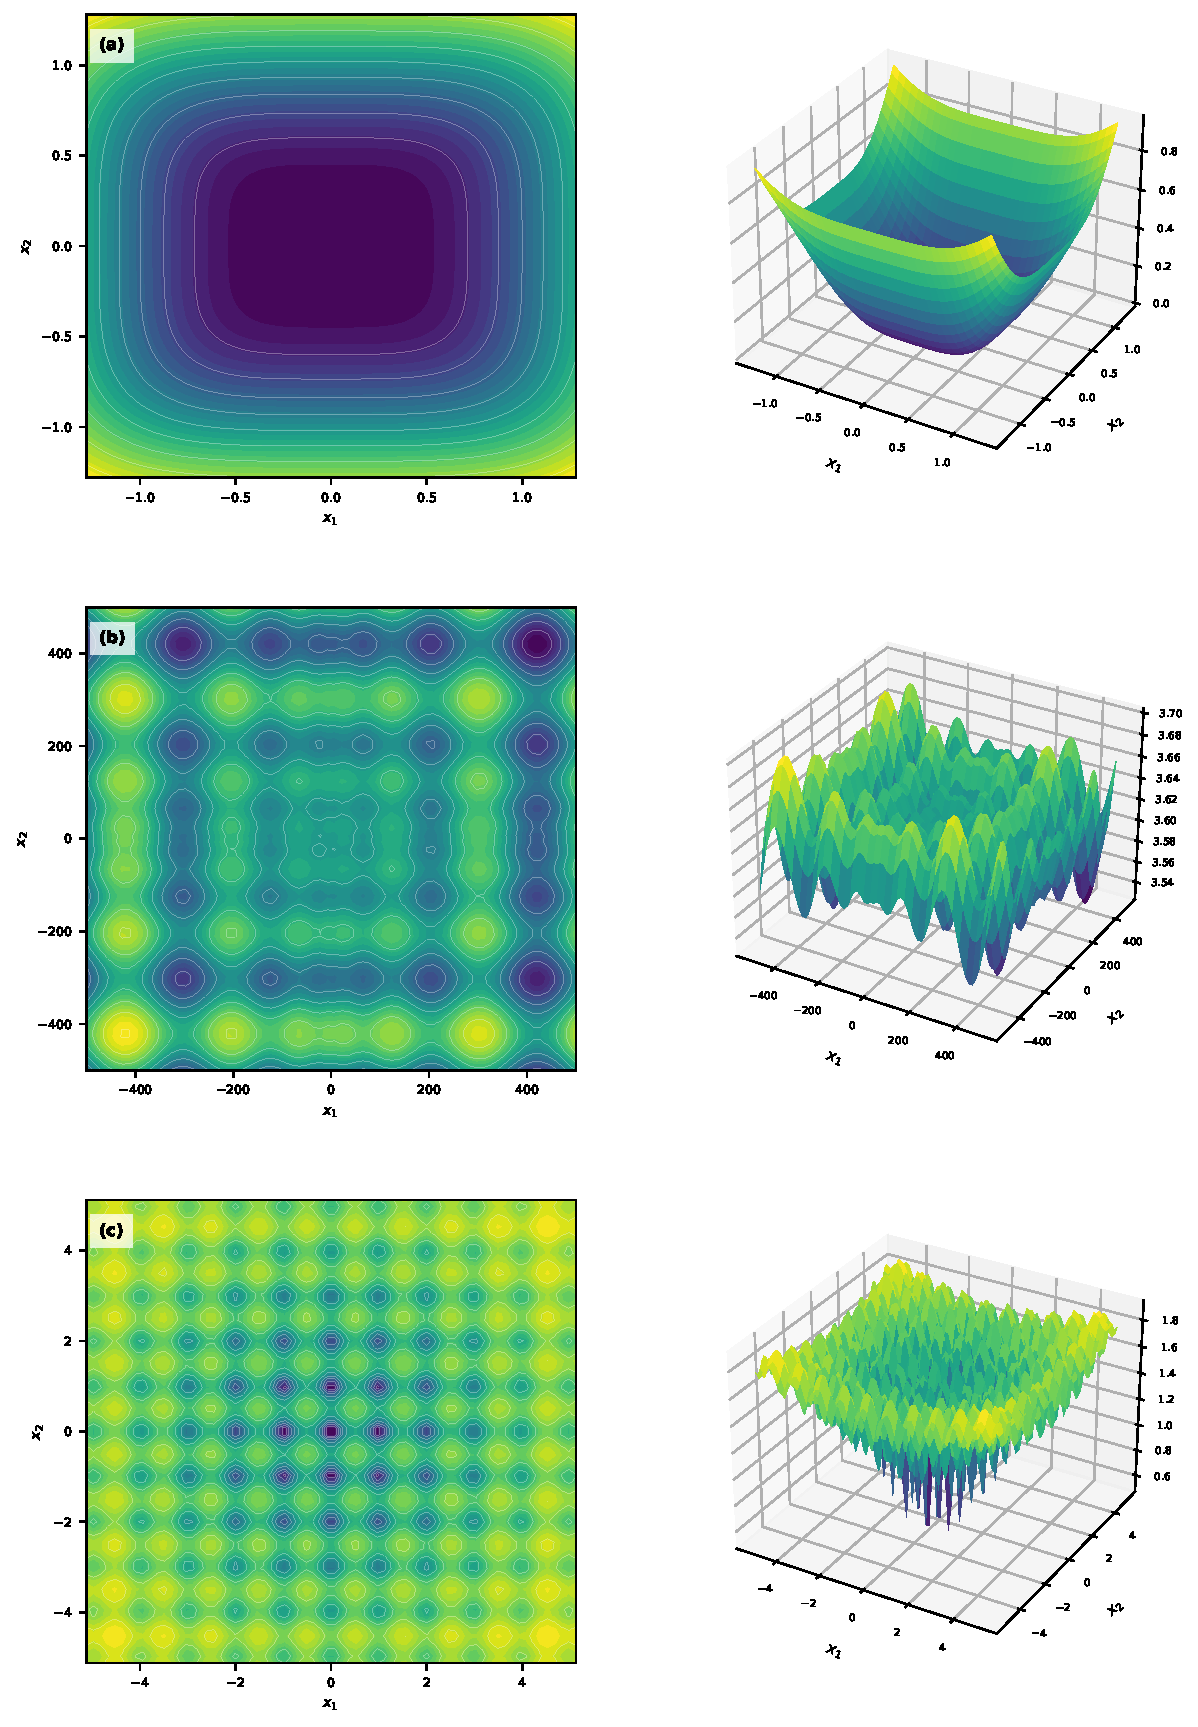
\includegraphics[width=\fulllength,height=0.84\textheight,keepaspectratio]{figures/landscapes_body/landscape_body_group_03.pdf}
  \end{adjustwidth}
  \caption{Benchmark objective landscapes and two-dimensional slices: (a) F7 (Quartic with noise, $d=10$); (b) F8 (Schwefel 2.26, $d=10$); (c) F9 (Rastrigin, $d=10$). Contours are shown at left and 3-D surfaces at right; colour shows log-compressed objective excess on function-specific scales. For $d>2$, other coordinates are fixed at the midpoint of the solver bounds. Bounds and reference optima are listed in Tables~\ref{tab:benchmark_scalable}--\ref{tab:benchmark_fixed}. The F7 panel uses the expected objective, including its 0.5 uniform-noise offset.}
  \label{fig:landscape_body_03}
\end{figure}
\clearpage

\begin{figure}[p]
  \begin{adjustwidth}{-\extralength}{0cm}
  \centering
  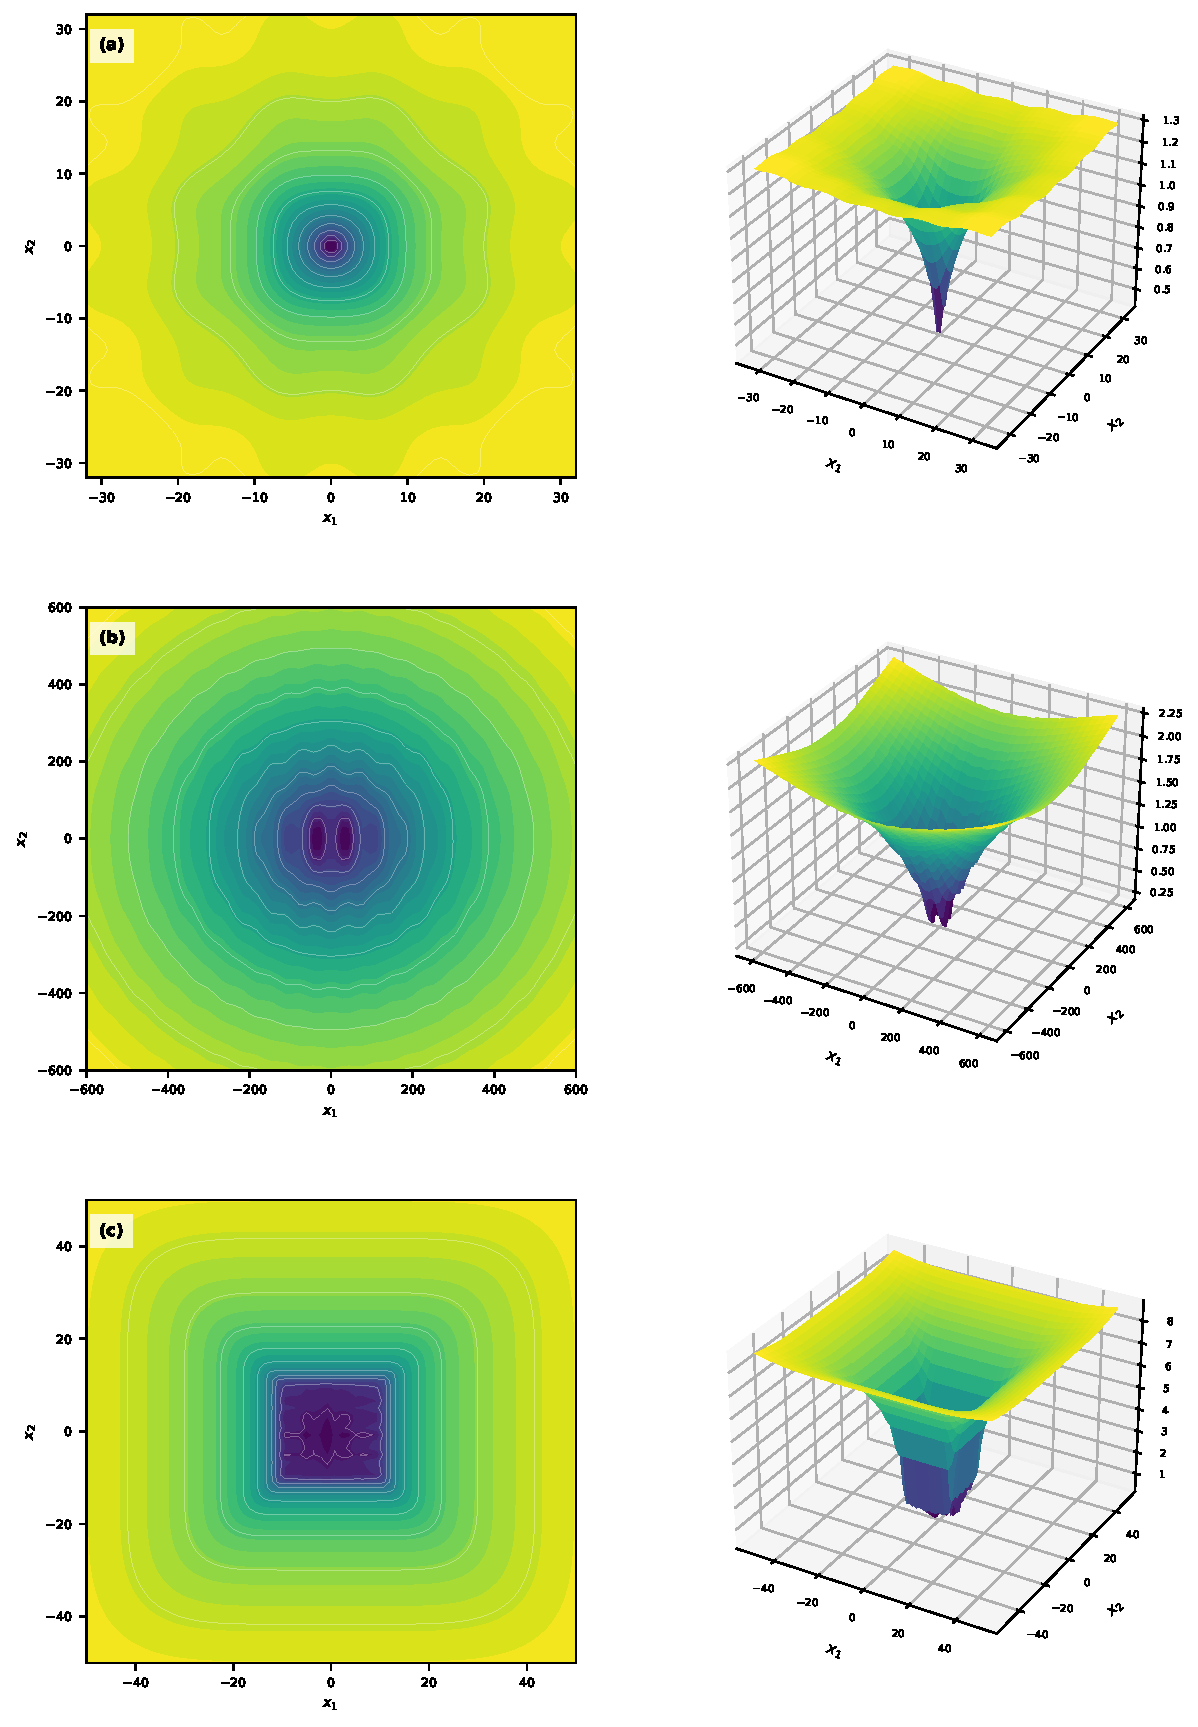
\includegraphics[width=\fulllength,height=0.84\textheight,keepaspectratio]{figures/landscapes_body/landscape_body_group_04.pdf}
  \end{adjustwidth}
  \caption{Benchmark objective landscapes and two-dimensional slices: (a) F10 (Ackley, $d=10$); (b) F11 (Griewank, $d=10$); (c) F12 (Penalized 1, $d=10$). Contours are shown at left and 3-D surfaces at right; colour shows log-compressed objective excess on function-specific scales. For $d>2$, other coordinates are fixed at the midpoint of the solver bounds. Bounds and reference optima are listed in Tables~\ref{tab:benchmark_scalable}--\ref{tab:benchmark_fixed}.}
  \label{fig:landscape_body_04}
\end{figure}
\clearpage

\begin{figure}[p]
  \begin{adjustwidth}{-\extralength}{0cm}
  \centering
  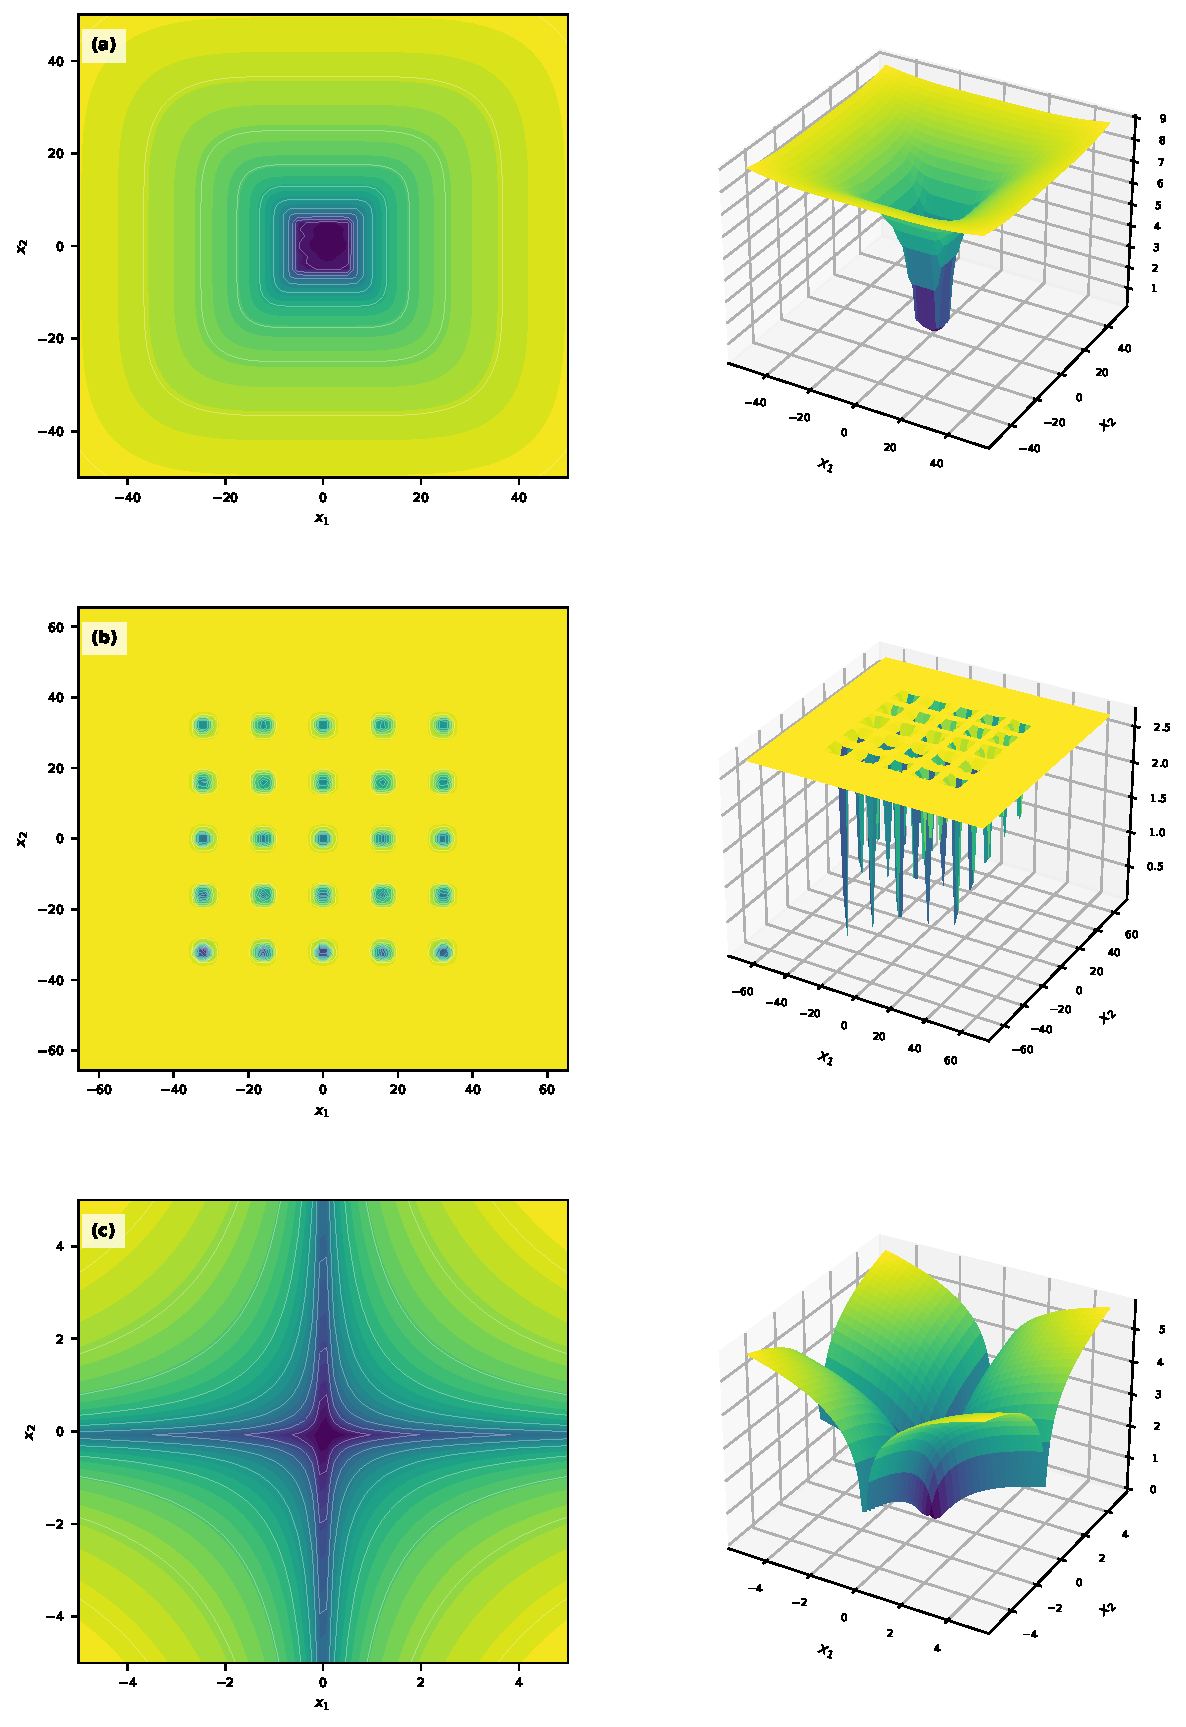
\includegraphics[width=\fulllength,height=0.84\textheight,keepaspectratio]{figures/landscapes_body/landscape_body_group_05.pdf}
  \end{adjustwidth}
  \caption{Benchmark objective landscapes and two-dimensional slices: (a) F13 (Penalized 2, $d=10$); (b) F14 (Shekel foxholes, $d=2$); (c) F15 (Kowalik, $d=4$). Contours are shown at left and 3-D surfaces at right; colour shows log-compressed objective excess on function-specific scales. For $d>2$, other coordinates are fixed at the midpoint of the solver bounds. Bounds and reference optima are listed in Tables~\ref{tab:benchmark_scalable}--\ref{tab:benchmark_fixed}.}
  \label{fig:landscape_body_05}
\end{figure}
\clearpage

\begin{figure}[p]
  \begin{adjustwidth}{-\extralength}{0cm}
  \centering
  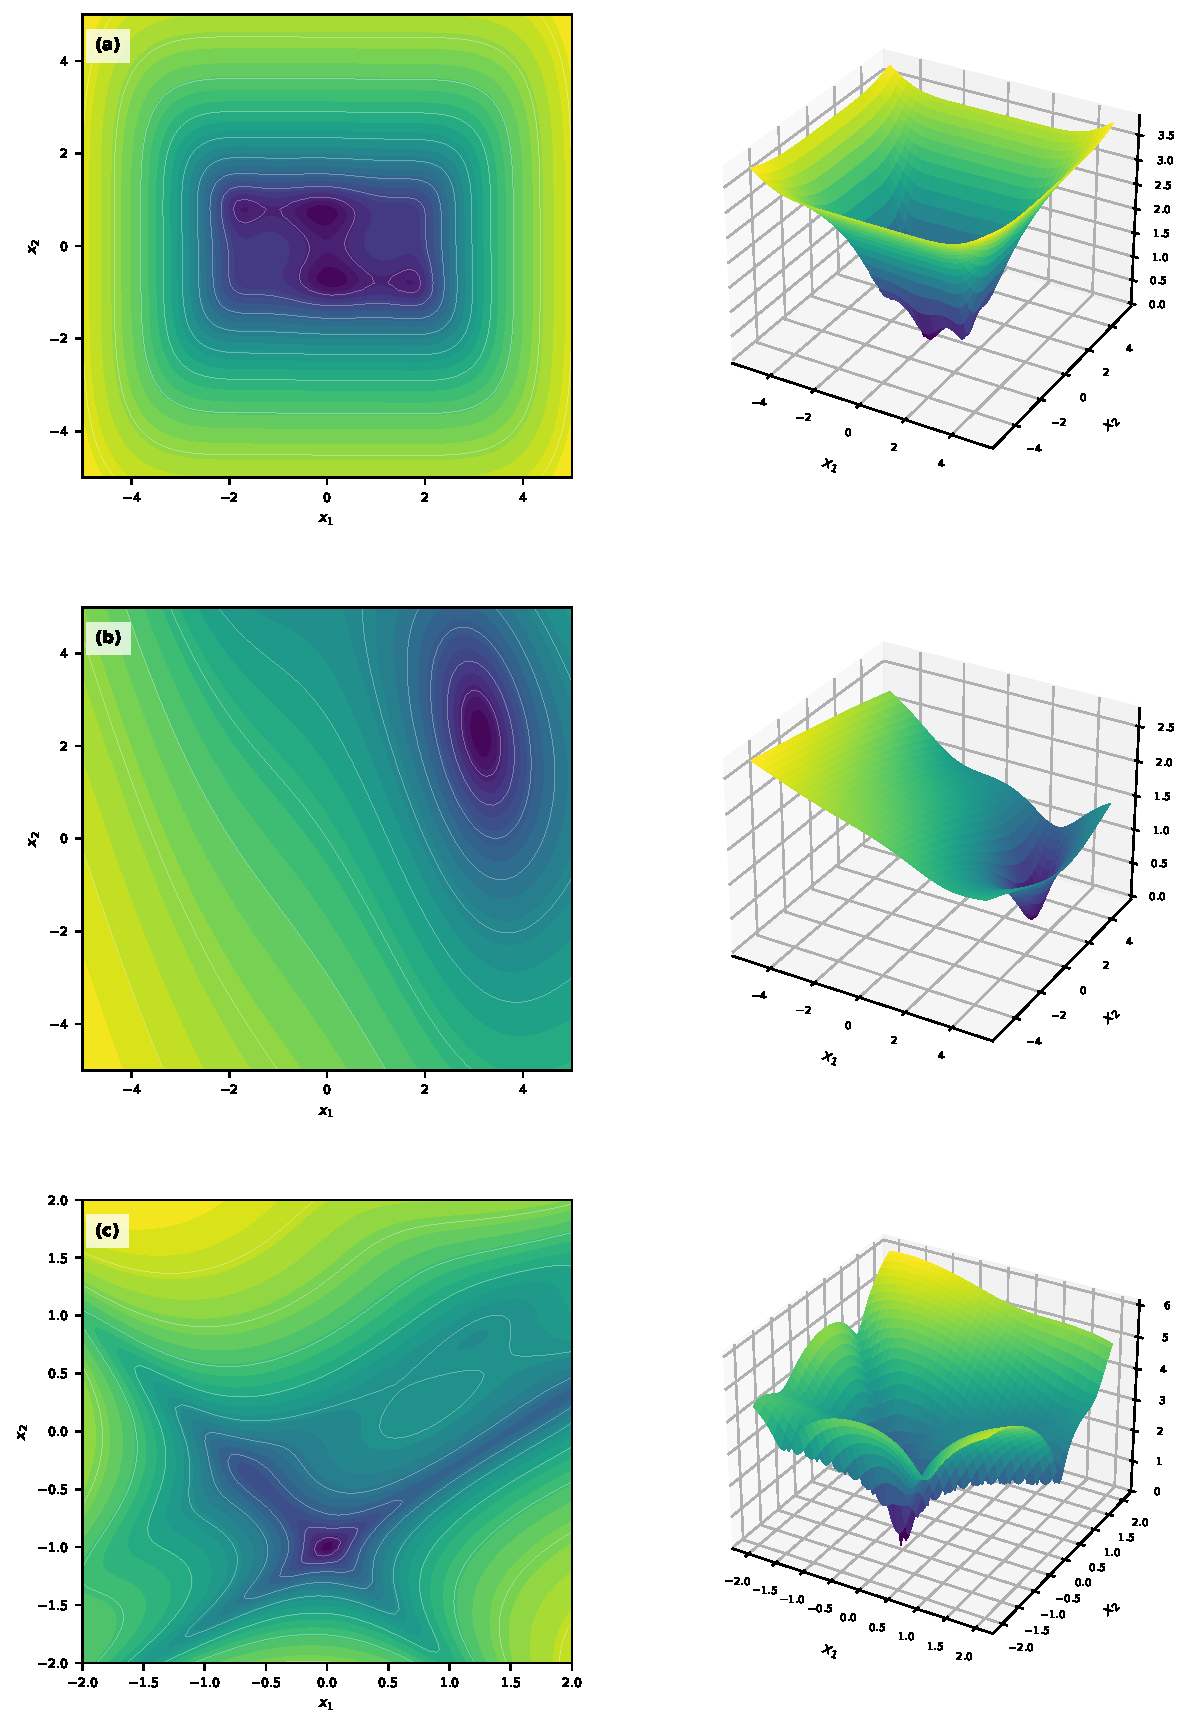
\includegraphics[width=\fulllength,height=0.84\textheight,keepaspectratio]{figures/landscapes_body/landscape_body_group_06.pdf}
  \end{adjustwidth}
  \caption{Benchmark objective landscapes and two-dimensional slices: (a) F16 (Six-hump camel, $d=2$); (b) F17 (Branin, $d=2$); (c) F18 (Goldstein-Price, $d=2$). Contours are shown at left and 3-D surfaces at right; colour shows log-compressed objective excess on function-specific scales. For $d>2$, other coordinates are fixed at the midpoint of the solver bounds. Bounds and reference optima are listed in Tables~\ref{tab:benchmark_scalable}--\ref{tab:benchmark_fixed}.}
  \label{fig:landscape_body_06}
\end{figure}
\clearpage

\begin{figure}[p]
  \begin{adjustwidth}{-\extralength}{0cm}
  \centering
  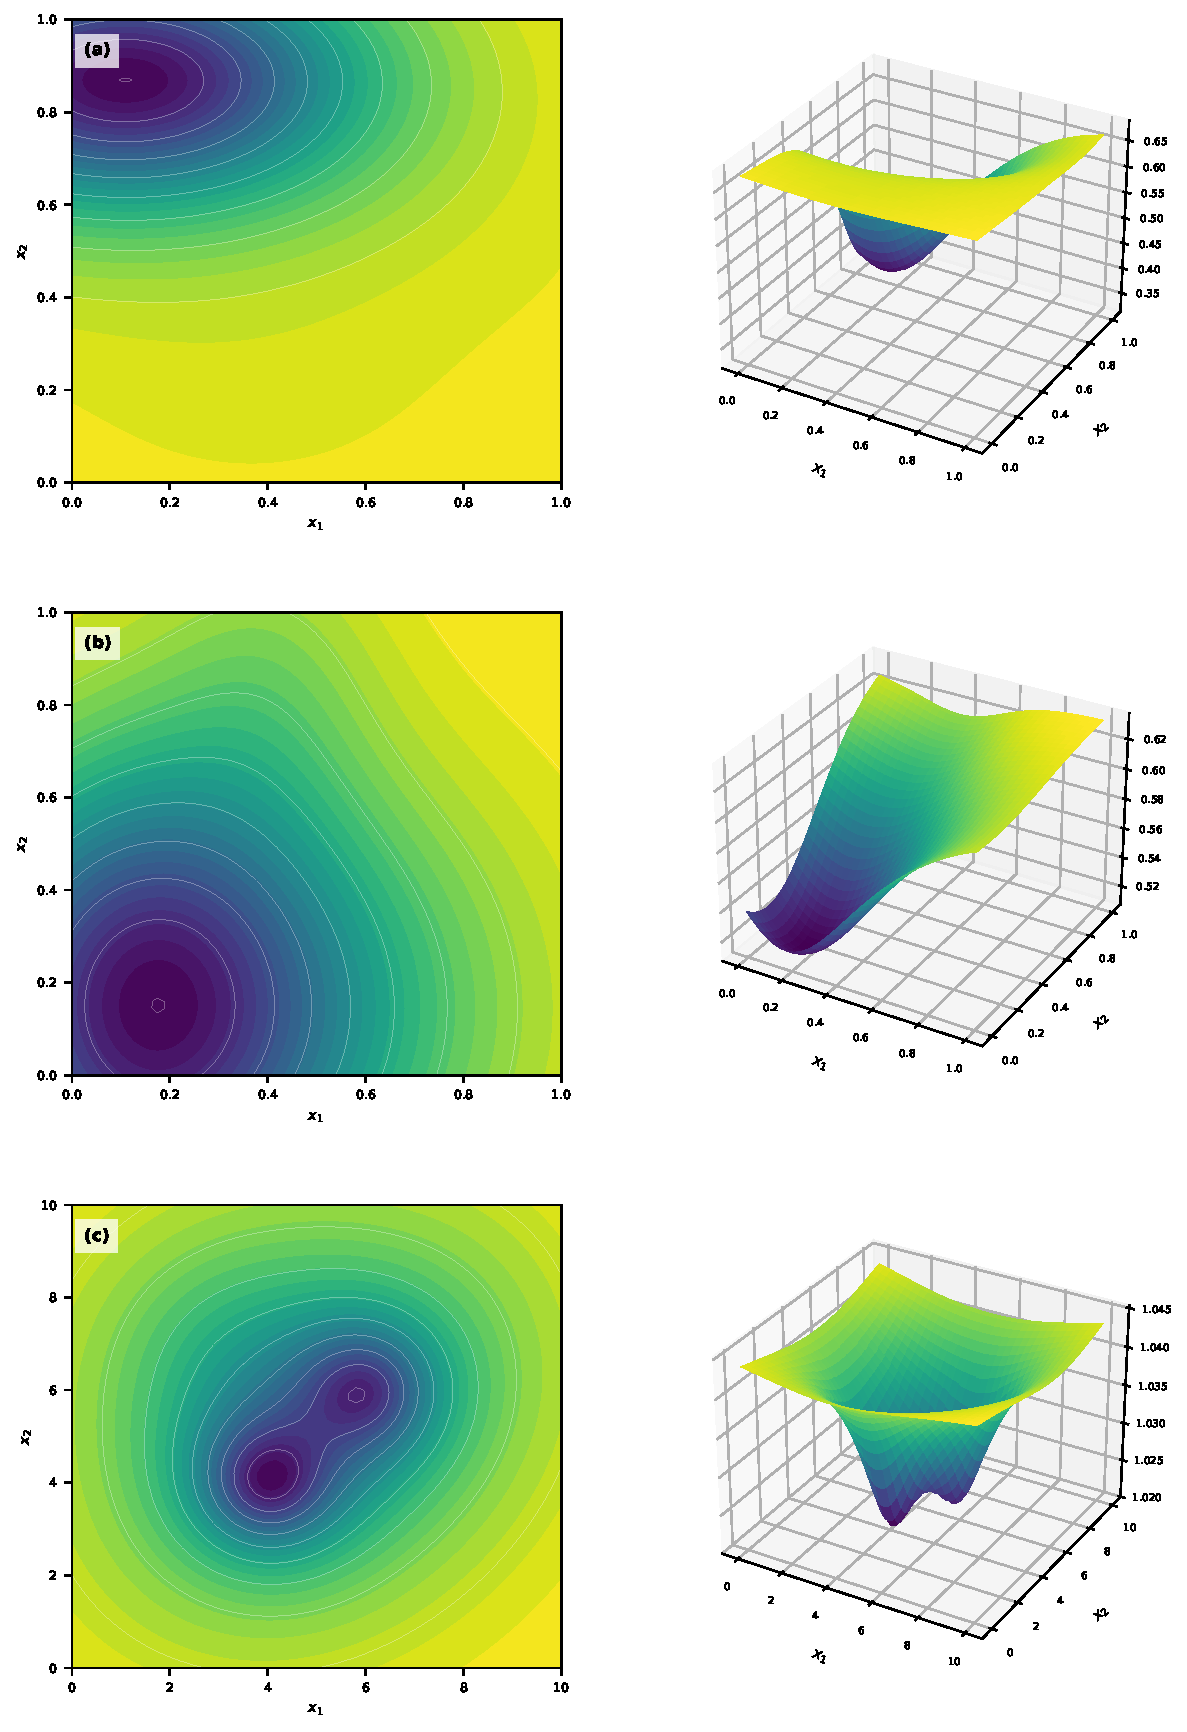
\includegraphics[width=\fulllength,height=0.84\textheight,keepaspectratio]{figures/landscapes_body/landscape_body_group_07.pdf}
  \end{adjustwidth}
  \caption{Benchmark objective landscapes and two-dimensional slices: (a) F19 (Hartmann 3-D, $d=3$); (b) F20 (Hartmann 6-D, $d=6$); (c) F21 (Shekel-5, $d=4$). Contours are shown at left and 3-D surfaces at right; colour shows log-compressed objective excess on function-specific scales. For $d>2$, other coordinates are fixed at the midpoint of the solver bounds. Bounds and reference optima are listed in Tables~\ref{tab:benchmark_scalable}--\ref{tab:benchmark_fixed}.}
  \label{fig:landscape_body_07}
\end{figure}
\clearpage

\begin{figure}[p]
  \begin{adjustwidth}{-\extralength}{0cm}
  \centering
  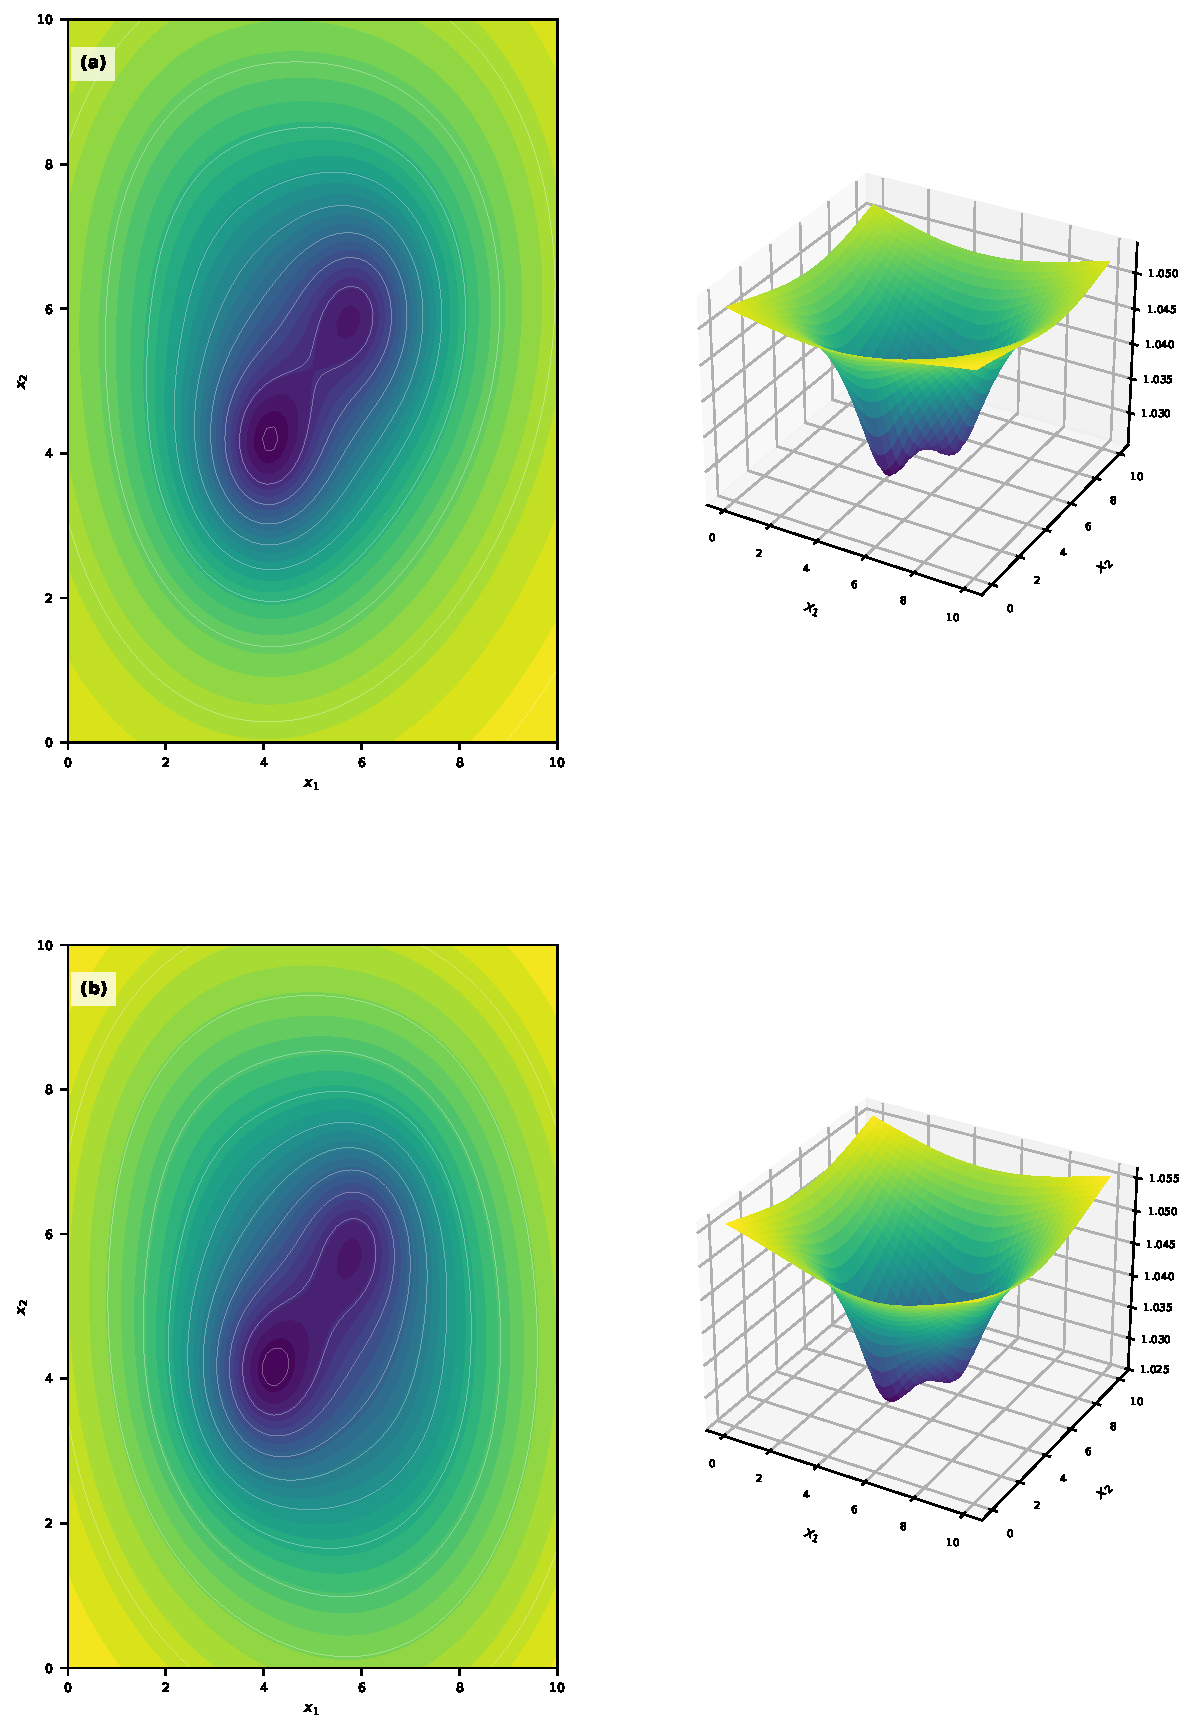
\includegraphics[width=\fulllength,height=0.84\textheight,keepaspectratio]{figures/landscapes_body/landscape_body_group_08.pdf}
  \end{adjustwidth}
  \caption{Benchmark objective landscapes and two-dimensional slices: (a) F22 (Shekel-7, $d=4$); (b) F23 (Shekel-10, $d=4$). Contours are shown at left and 3-D surfaces at right; colour shows log-compressed objective excess on function-specific scales. For $d>2$, other coordinates are fixed at the midpoint of the solver bounds. Bounds and reference optima are listed in Tables~\ref{tab:benchmark_scalable}--\ref{tab:benchmark_fixed}.}
  \label{fig:landscape_body_08}
\end{figure}
\clearpage
